\begin{frame}
    \shiftedframetitle{Content}
   
   
\begin{minipage}{0.35\textwidth}
{\large
    \begin{enumerate}
     \itemsep3ex
    \item<2-> Introduction
%    \begin{itemize}
%    \setlength{\itemindent}{1cm}
%	    \item Previous work
%    \end{itemize}
    \item<3-> Theory 
%	\begin{itemize}
%	\setlength{\itemindent}{1cm}
%		\item Shallow Water Equations model 
%	\end{itemize}
%    \item<4->  Tools 
%    	\begin{itemize}
%    	\setlength{\itemindent}{1cm}
%		\item interFoam
%		\item SWE solver 
%	\end{itemize}
    \item<4-> Implementation
    \item<5-> Results
    \item<6-> Conclusions
%    	\begin{itemize}
%    	\setlength{\itemindent}{1cm}
%		\item Future research
%	\end{itemize}
    \end{enumerate}
}
\end{minipage}
\begin{minipage}{0.4\textwidth}
     \begin{figure}
     \includegraphics[scale=0.325]{Resources/Images/imagesThesis/presentation_swe_of_sup47}
     \end{figure}
\end{minipage}   
\end{frame}
\clearpage

%%%%%%%%%%%%%%%%%%%%
%%%%%%%%%%%%%%%%%%%%%
%\begin{frame}
%\shiftedframetitle{1. Introduction}
%\begin{itemize}
%\item abstract
%\item previous work
%\item motivation of the thesis
%% \vspace{3em}
%% \begin{itemize}
%%  \setlength\itemsep{2em}
%%  \item  full description of \myTUMdarkblue{\textit{shallowFOAM}}  solver for \myTUMdarkblue{$2D$} SWE \cite{mintgen}
%% \item  \myTUMdarkblue{coupling $2D$} SWE and \myTUMdarkblue{$3D$} RANS solvers $\rightarrow$ development of \textit{shallowInterFOAM} \cite{mintgen}
%% \item B.Sc. Christiaan Osse implemented \cite{mintgen} with \myTUMdarkblue{\textit{preCICE}}
%\end{itemize}
%\end{frame}
%\clearpage

 %%%%%%%%%%%%%%%%%%%%%%%%%%
%%%%%%%%%%%%%%%%%%%%%%%%%%

\begin{frame}
\shiftedframetitle{1. Introduction}
%\begin{itemize}
%\item Cases \cite{espinosa}
%\item mapping
%\item Boundary conditions
%\end{itemize}
{\Large \textbf{Idea...}}\\[1.5cm]
\hspace{1cm}
\begin{minipage}{0.35\textwidth}
\begin{tcolorbox}[
colframe=TUMDarkBlue,
%colback=TUMDarkBlue!50,
title = \centering SWE\\2D] 
\begin{itemize}
\setlength\itemsep{1em}
\item[+] Simpler model 
\item[+] $O(n^2)$
\item[-] Valid when $H/L \leq 0.05$ %\vspace{1cm}
\item[-] 3D effects neglected. \vspace{0.5cm}
\end{itemize}
\end{tcolorbox}    
\end{minipage}
\begin{minipage}{0.15\textwidth}
\hspace{0.5cm}
%\vspace{-0.5cm}
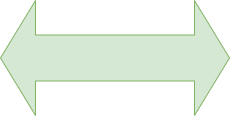
\includegraphics[width=1\textwidth]{Resources/Images/arrow2.png}\\
\end{minipage}
\begin{minipage}{0.35\textwidth}
%\vspace{0cm}
\begin{tcolorbox} [
colframe=TUMOrange,
%colback=TUMOrange!50,
title = \centering Navier-Stokes\\3D]     
\begin{itemize}
\setlength\itemsep{1em}
\item[+] 3D effects are caught
\item[-] large number of cells for low accuracy results
\item[-] $O(n^3)$\vspace{0.6cm}
\end{itemize}
\end{tcolorbox}    
\end{minipage}


% \item<4-> \myCRed{Extend} \cite{mintgen} coupling ($2D$ $\leftrightarrow$ $3D$) as a \myCRed{flexible} approach to SWE solvers\\[2em]
% \item<5-> Test Case: $2D$ SWE solver \& OpenFOAM\\[2em]
% \item<6-> \myCRed{Coupling} \& \myCRed{Mapping} data from/to all setups: \vspace{0.4cm}
%\begin{table}[]
%\begin{tabular}{|lll|}\hline
%$2D$ SWE       & $\rightarrow$ & $2D$ SWE       \\ \hline
%$2D$ SWE       & $\rightarrow$ & $3D$ OpenFOAM \\ \hline
%$3D$ OpenFOAM & $\rightarrow$ & $2D$ SWE       \\ \hline
%$3D$ OpenFOAM & $\rightarrow$ & $3D$ OpenFOAM \\ \hline
%\end{tabular}
%\caption{Mapping setups}
%\label{table:1}
%\end{table}
%\item<7-> \textbf{\textit{\myCRed{Extend preCICE} adapter for handling $2D\leftrightarrow3D$ domains}}
%\end{itemize}
 \end{frame}



%%%%%%%%%%%%%%%%%%%%%%%%%%
%%%%%%%%%%%%%%%%%%%%%%%%%%

\begin{frame}
\shiftedframetitle{1. Introduction}
%\begin{itemize}
%\item Cases \cite{espinosa}
%\item mapping
%\item Boundary conditions
%\end{itemize}
%\hspace{0.5cm}
\begin{minipage}{0.3\textwidth}
\begin{itemize}
\item<1->[] {\Large \textbf{Previous work}}\\[1.5cm]
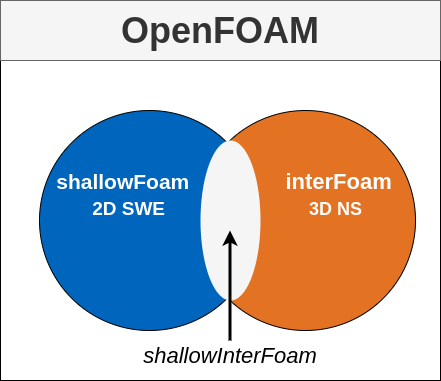
\includegraphics[width=1\textwidth]{Resources/Images/Mintgenwork.png}
\end{itemize}
\end{minipage}
\hspace{3cm}
\begin{minipage}{0.5\textwidth}
\vspace{-2.2cm}
\begin{itemize}
\item<2->[] {\Large \textbf{This work}}\\[3cm]
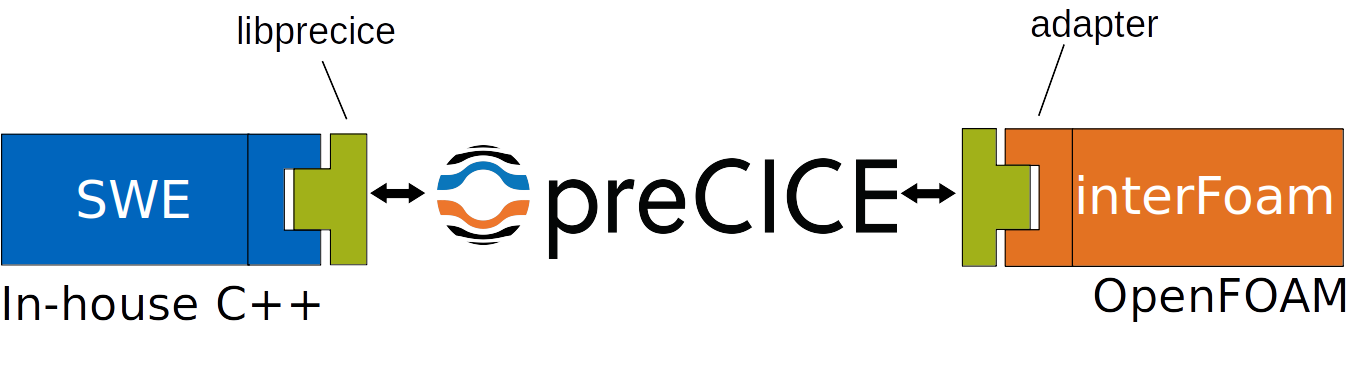
\includegraphics[width=1\textwidth]{Resources/Images/pash2.png}
%\vspace*{\fill}
\end{itemize}
\end{minipage}


%\item<3->[]
%\hspace{0.35\columnwidth}{\large\textbf{Goals}}
%\vspace{3em}
% \begin{itemize}
%
% \item<4-> \myCRed{Extend} \cite{mintgen} coupling ($2D$ $\leftrightarrow$ $3D$) as a \myCRed{flexible} approach to SWE solvers\\[2em]
% \item<5-> Test Case: $2D$ SWE solver \& OpenFOAM\\[2em]
% \item<6-> \myCRed{Coupling} \& \myCRed{Mapping} data from/to all setups: \vspace{0.4cm}
%\begin{table}[]
%\begin{tabular}{|lll|}\hline
%$2D$ SWE       & $\rightarrow$ & $2D$ SWE       \\ \hline
%$2D$ SWE       & $\rightarrow$ & $3D$ OpenFOAM \\ \hline
%$3D$ OpenFOAM & $\rightarrow$ & $2D$ SWE       \\ \hline
%$3D$ OpenFOAM & $\rightarrow$ & $3D$ OpenFOAM \\ \hline
%\end{tabular}
%\caption{Mapping setups}
%\label{table:1}
%\end{table}
%\item<7-> \textbf{\textit{\myCRed{Extend preCICE} adapter for handling $2D\leftrightarrow3D$ domains}}
%\end{itemize}
 \end{frame}
 
 
 
